  \documentclass[final]{beamer} % beamer 3.10: do NOT use option hyperref={pdfpagelabels=false} !
%\documentclass[final,hyperref={pdfpagelabels=false}]{beamer} % beamer 3.07: get rid of beamer warnings
\mode<presentation> {  %% check http://www-i6.informatik.rwth-aachen.de/~dreuw/latexbeamerposter.php for examples
	\usetheme{I6dv}    %% you should define your own theme e.g. for big headlines using your own logos 
}
\usepackage[english]{babel}
\usepackage[latin1]{inputenc}
\usepackage{amsmath,amsthm, amssymb, latexsym}
%\usepackage{times}\usefonttheme{professionalfonts}  % times is obsolete
\usefonttheme[onlymath]{serif}
\boldmath
\usepackage[orientation=landscape,size=a1,scale=1.4,debug]{beamerposter}                       % e.g. for DIN-A0 poster
%\usepackage[orientation=portrait,size=a1,scale=1.4,grid,debug]{beamerposter}                  % e.g. for DIN-A1 poster, with optional grid and debug output
%\usepackage[size=custom,width=200,height=120,scale=2,debug]{beamerposter}                     % e.g. for custom size poster
%\usepackage[orientation=portrait,size=a0,scale=1.0,printer=rwth-glossy-uv.df]{beamerposter}   % e.g. for DIN-A0 poster with rwth-glossy-uv printer check
% ...
%
\title[Fancy Posters]{Prometheus AI}
\author{Sean Stappas}
\institute[RWTH Aachen University]{McGill University}
\date{Jul. 31th, 2007}

% edit this depending on how tall your header is. We should make this scaling automatic :-/
\newlength{\columnheight}
\setlength{\columnheight}{104cm}


\begin{document}
\begin{columns}
	\begin{column}{.3\textwidth}
			\begin{block}{Introduction}
				\begin{figure}[!htb]
					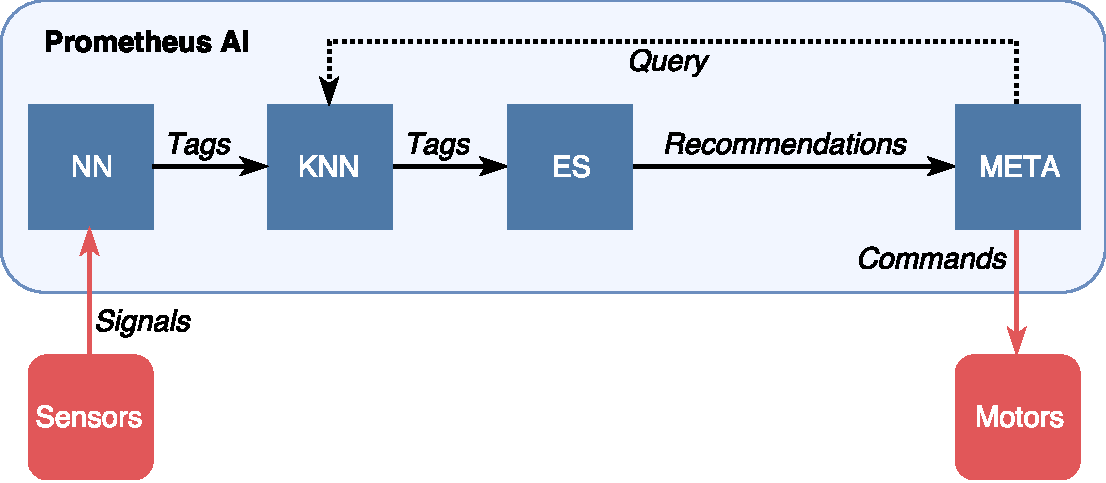
\includegraphics[width=\textwidth]{figures/ai_model_labeled.pdf}
					\caption{Prometheus AI model with labeled input and output.}
					\label{model_labeled}
				\end{figure}
			\end{block}
			\begin{block}{Problem}
				\begin{figure}[!htb]
					\centering
					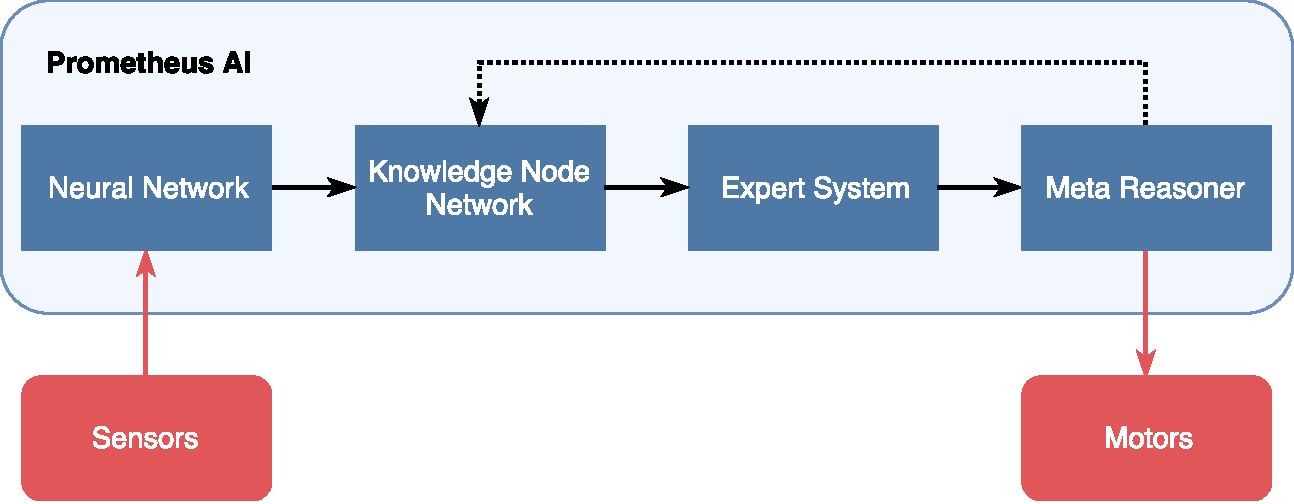
\includegraphics[width=0.5\columnwidth]{figures/ai_model.pdf}
					\caption
					{Test circuit 1 with labeled nodes.}
				\end{figure}
			\end{block}
	\end{column}
	\begin{column}{.3\textwidth}
		\begin{block}{Design}
			
			\begin{figure}[!htb]
				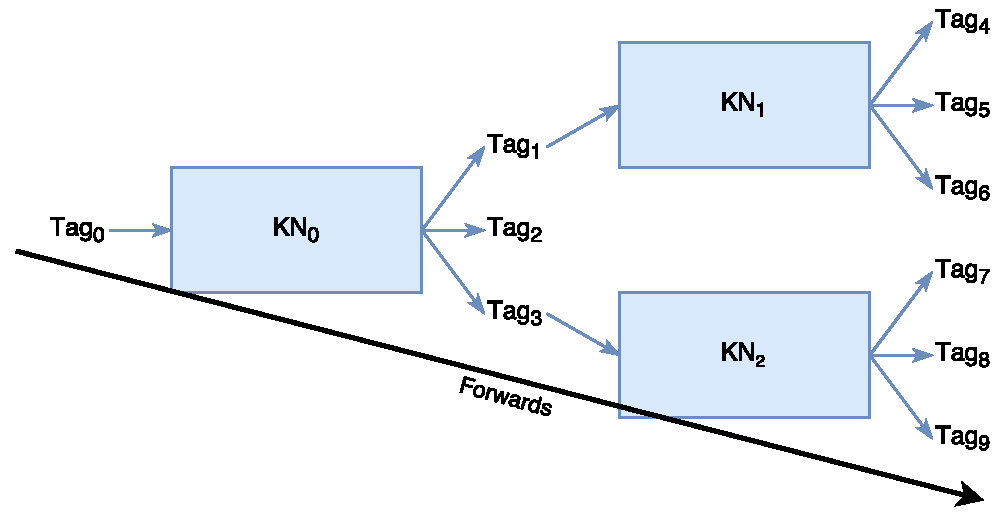
\includegraphics[width=0.5\columnwidth]{figures/forwards_thinking.pdf}
				\caption{Thinking forwards in the KNN.}
				\label{think_forwards}
			\end{figure}
		
			\begin{figure}[!htb]
				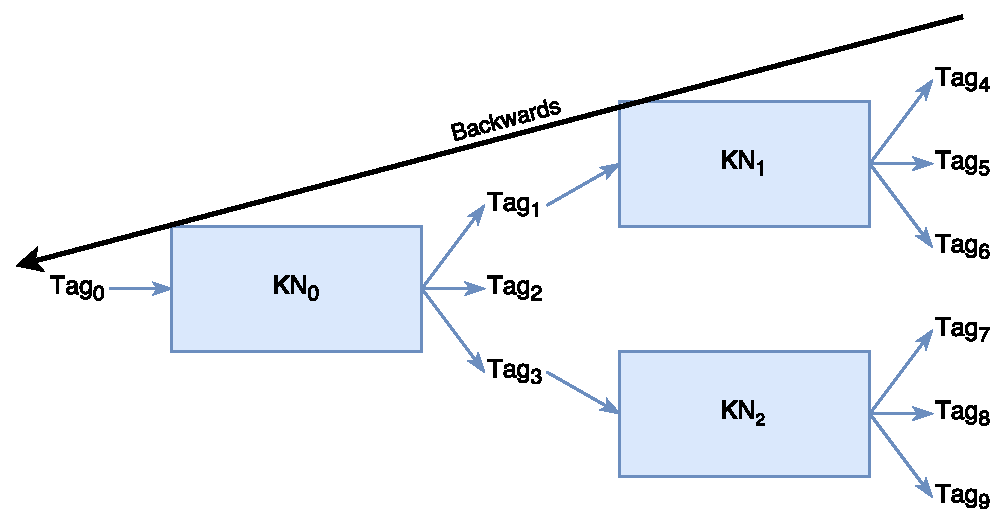
\includegraphics[width=0.5\columnwidth]{figures/backwards_thinking.pdf}
				\caption{Thinking backwards in the KNN.}
				\label{think_backwards}
			\end{figure}
		
			\begin{figure}[!htb]
				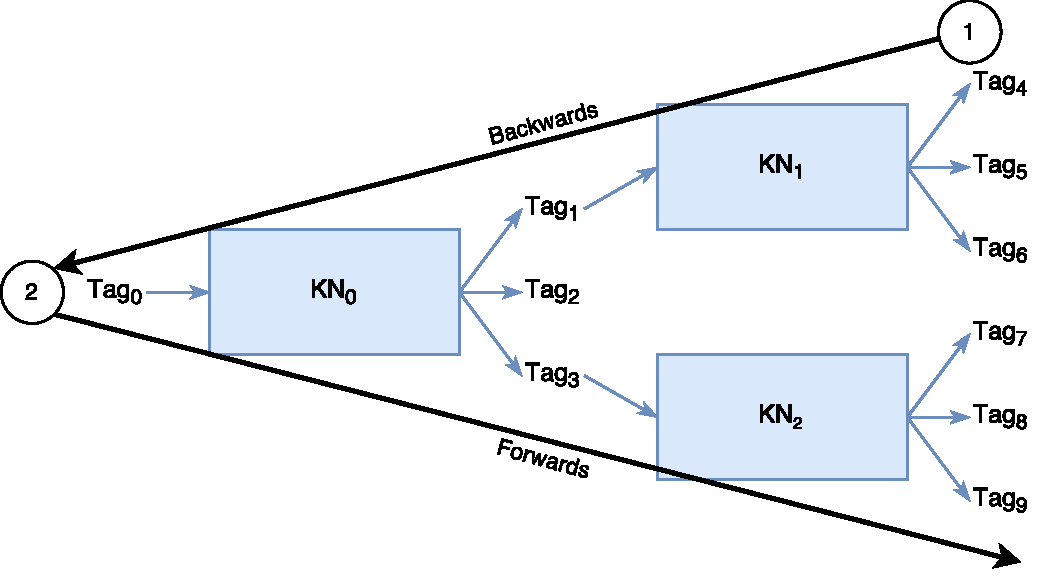
\includegraphics[width=0.5\columnwidth]{figures/lambda_thinking.pdf}
				\caption{Lambda thinking in the KNN.}
				\label{think_lambda}
			\end{figure}
		\end{block}
	\end{column}
	\begin{column}{.3\textwidth}
	\begin{block}{Implementation}
		\begin{figure}[!htb]
			\centering
			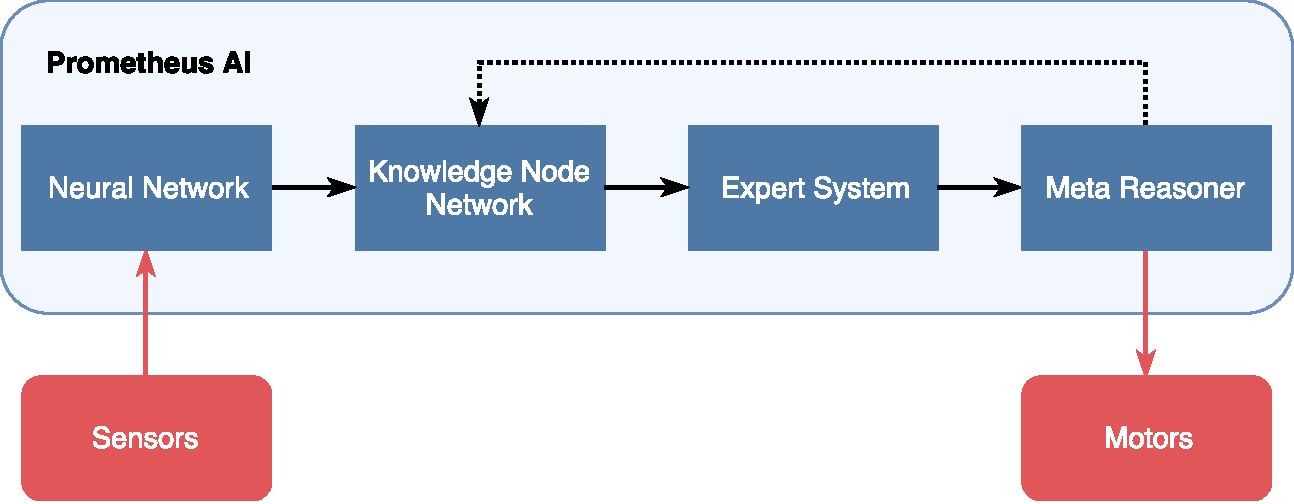
\includegraphics[width=0.5\columnwidth]{figures/ai_model.pdf}
			\caption
			{Test circuit 1 with labeled nodes.}
		\end{figure}
	\end{block}
	\end{column}
\end{columns}
\end{document}